\documentclass[10pt,a4paper]{article}
\usepackage[utf8]{inputenc}
\usepackage{amsmath}
\usepackage{amsfonts}
\usepackage{amssymb}
\usepackage{makeidx}
\usepackage{graphicx}
\usepackage{parskip}
\usepackage[left=2cm,right=2cm,top=2cm,bottom=2cm]{geometry}
\author{Miguel Angel Xamie Diaz Fuentes/Jimenez Cortes Raul}

\begin{document}
\begin{center}
\begin{LARGE}
\textbf{INGENIERÍA MECATRÓNICA}\\
\end{LARGE}
{\large Sistemas Electrónicos De Interfaz}\\

\begin{figure}[hbtp]
\centering

\includegraphics[scale=0.80]{UPZMG_Mecatr_nica.png}
\end{figure} 

\begin{center}
\begin{LARGE}
EV-2-5 ARREGLOS DE AMPLIFICADORES DE POTENCIA
\end{LARGE}
\end{center}

\begin{Large}
\textbf{Alumno}
\\\textit{Miguel Angel Xamie Diaz Fuentes\\Raul Jimenez Cortez}
\textbf{\\Maestro}
\\\textit{Morán Garabito Carlos Enrique}
\textbf{\\Fecha de Entrega}
\\\textit{08/11/2019}
\textbf{\\Grupo}
\\\textit{4-B}\\
\textbf{Período Cuatrimestral}\\
\textit{2019-Septiembre-Diciembre}
\\
\end{Large}

\end{center}

\footnote{Universidad Politécnica De La Zona Metropolitana De Guadalajara} 

\newpage

\section{Marco Teórico}
\textbf{AMPLIFICADOR OPERACIONAL}\\
Un amplificador operacional, a menudo conocido op-amp por sus siglas en inglés (operational amplifier) es un dispositivo amplificador electrónico de alta ganancia acoplado en corriente continua que tiene dos entradas y una salida. En esta configuración, la salida del dispositivo es, generalmente, de cientos de miles de veces mayor que la diferencia de potencial entre sus entradas.\\

\textbf{CARACTERISTICAS DEL AMPLIFICADOR OPERACIONAL}\\

\textbf{Amplificador operacional ideal}\\
-Corriente de entrada cero.
-Voltaje de desequilibrio de entrada cero.
-Infinito rango de voltaje disponible en la salida.
-Infinito ancho de banda con desplazamiento de fase cero.
-Rapidez de variación de voltaje infinita.
-Ruido cero.
Infinito rechazo de modo común (CMRR)
-Infinito factor de rechazo a fuente de alimentación (PSRR).
Estas características se pueden resumir en dos "reglas de oro":
-En el lazo cerrado la salida intenta hacer lo necesario para hacer cero la diferencia de voltaje entre las entradas.
-Las corrientes de entrada al dispositivo son cero.3\\

\textbf{Amplificador operacional real}\\
El amplificador real difiere del ideal en varios aspectos:
-Ganancia en lazo abierto, para corriente continua, desde 100.000 hasta más de 1.000.000.
-Resistencia de entrada finita, desde 0,3 MOHMS en adelante.
-Resistencia de salida no cero.
-Corriente de entrada no cero, generalmente de 10 nA en circuitos de tecnología bipolar.
-Voltaje de desequilibrio de entrada no cero, en ciertos dispositivos es de 15 mV
-Rechazo de modo común no infinito, aunque grande, en algunos casos, de 80 a 95 dB.
-Rechazo a fuente de alimentación no infinito.
-Características afectadas por la temperatura de operación.
-Deriva de las características, debido al envejecimiento del dispositivo.
-Ancho de banda finito, limitado a propósito por el diseño o por características de los materiales.
-Presencia de ruido térmico.
-Presencia de efectos capacitivos en la entrada por la cercanía de los terminales entre sí.
-Corriente de salida limitada.
-Potencia disipada limitada.\\

\textbf{AMPLIFICADOR INVERSOR}\\
Se llama así este montaje porque la señal de salida es inversa de la de entrada, en polaridad, aunque pude ser mayor, igual o menor, dependiendo esto de la ganancia que le demos al amplificador en lazo cerrado. La señal, como vemos en la figura, se aplica al terminal inversor o negativo del amplificador y el positivo o no inversor se lleva a masa.\\

\textbf{AMPLIFICADOR NO INVERSOR}\\
El amplificador no-Inversor es una configuración que permite amplificar una señal electrónica. Entonces su caracteristica, no altera la fase de entrada. Recordemos que un amplificador operacional tiene 2 entradas y una salida, la entrada positiva o no-inversora y la negativa o entrada inversora. Por ejemplo, la configuración se realiza mediante dos resistencias conectadas. Por lo tanto las resistencia se conectan a la entrada negativa y salida. Mientras que la señal de entrada se conecta a la entrada no-inversora.\\

\textbf{SUMADOR DE TRES SEÑALES CON AMPLIFICADOR OPERACIONAL}\\
El amplificador sumador con amplificadores operacionales entrega en su salida un voltaje igual a la suma de los voltajes que tiene en sus entradas. La explicación siguiente se basa en un sumador de tres entradas, pero aplica para un sumador de cualquier número de entradas.\\

\textbf{AMPLIFICADOR RESTADOR}\\
Este amplificador usa ambas entradas invertida y no invertida con una ganancia de uno, para producir una salida igual a la diferencia entre las entradas. Es un caso especial del amplificador diferencial. Se pueden elegir tambien las resistencias para amplificar la diferencia. \\












\footnote{Universidad Politécnica De La Zona Metropolitana De Guadalajara} 

\newpage

\section{Primer Circuito}
\begin{center}
 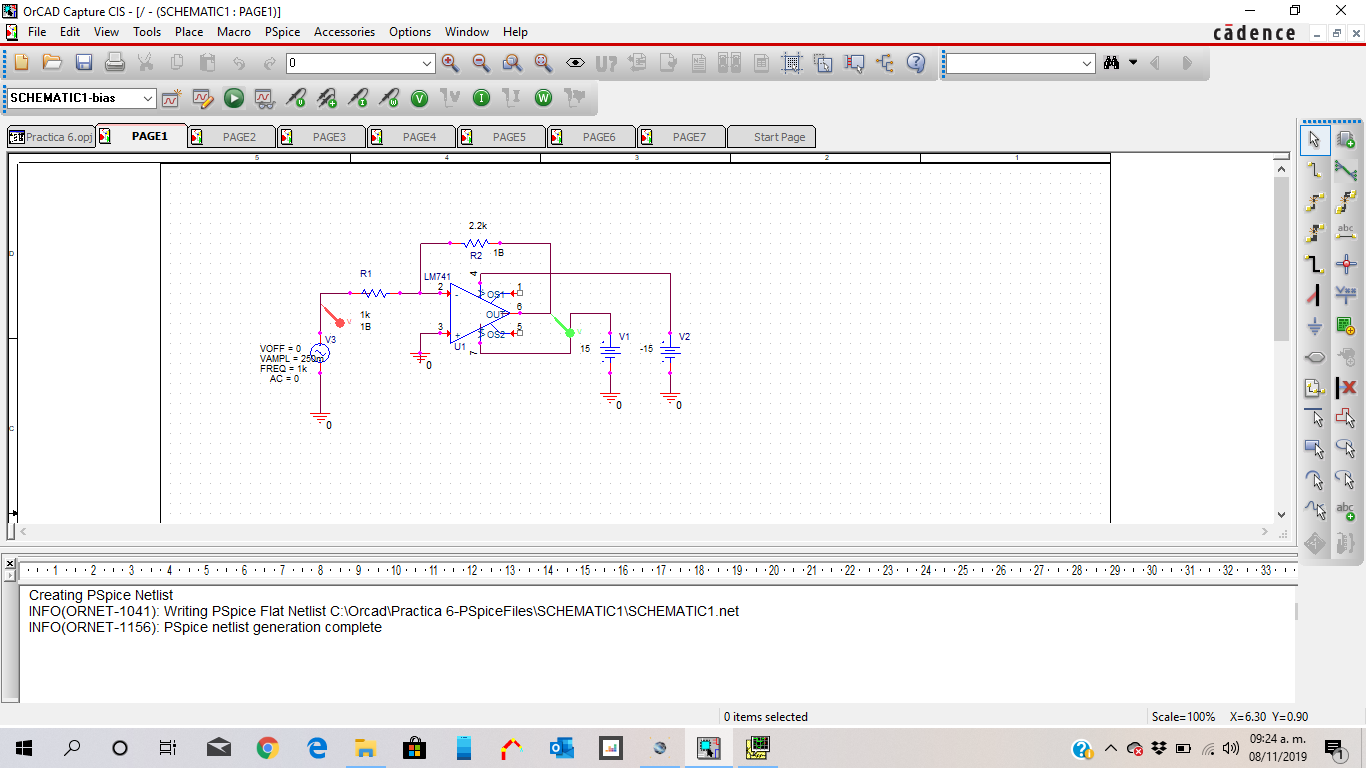
\includegraphics[scale=0.3]{1.png}
 \begin{figure}[hbtp]
 \caption{Amplificador Operacional Inversor}
 \centering
 \end{figure}\\
  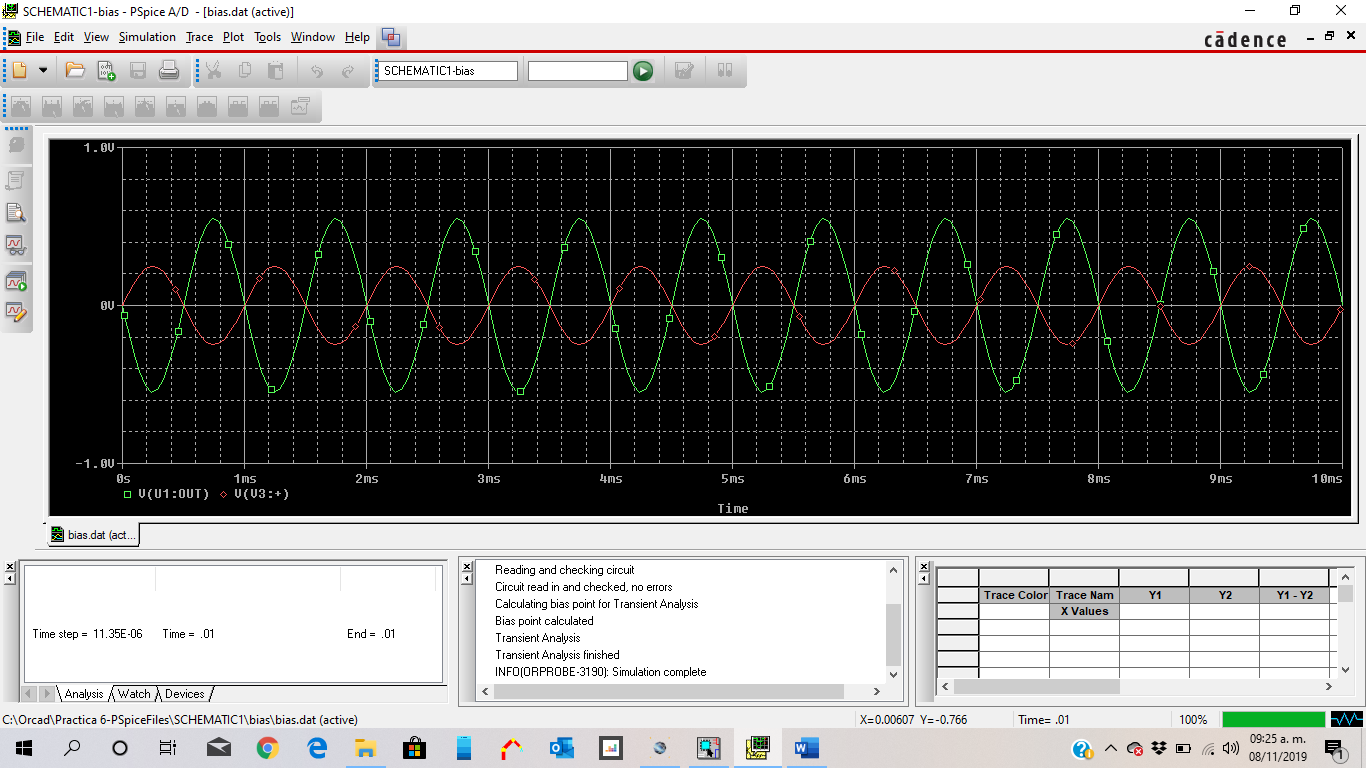
\includegraphics[scale=0.3]{2.png}
 \begin{figure}[hbtp]
 \caption{Simulacion}
 \centering
 \end{figure} 
\end{center}

En la simulacion se puede apreciar el cual es un inversor donde tambien muestra su ganancia en donde es 2.2/1= \textbf{2.2} es su ganacia.

\subsection{Preguntas PDF}
















\footnote{Universidad Politécnica De La Zona Metropolitana De Guadalajara} 

\newpage

\section{Segundo Circuito}
\begin{center}
 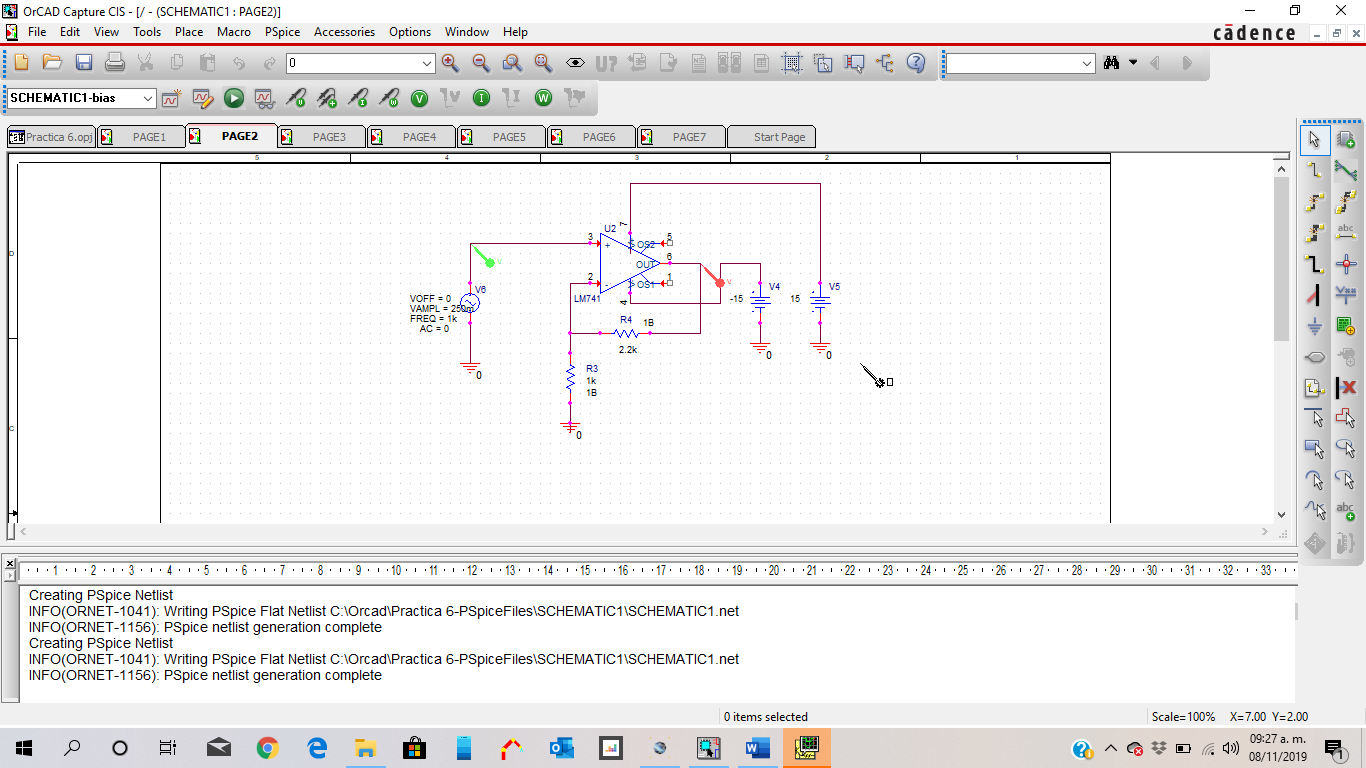
\includegraphics[scale=0.3]{3.png}
 \begin{figure}[hbtp]
 \caption{Amplificador Operacional No Inversor}
 \centering
 \end{figure}\\
  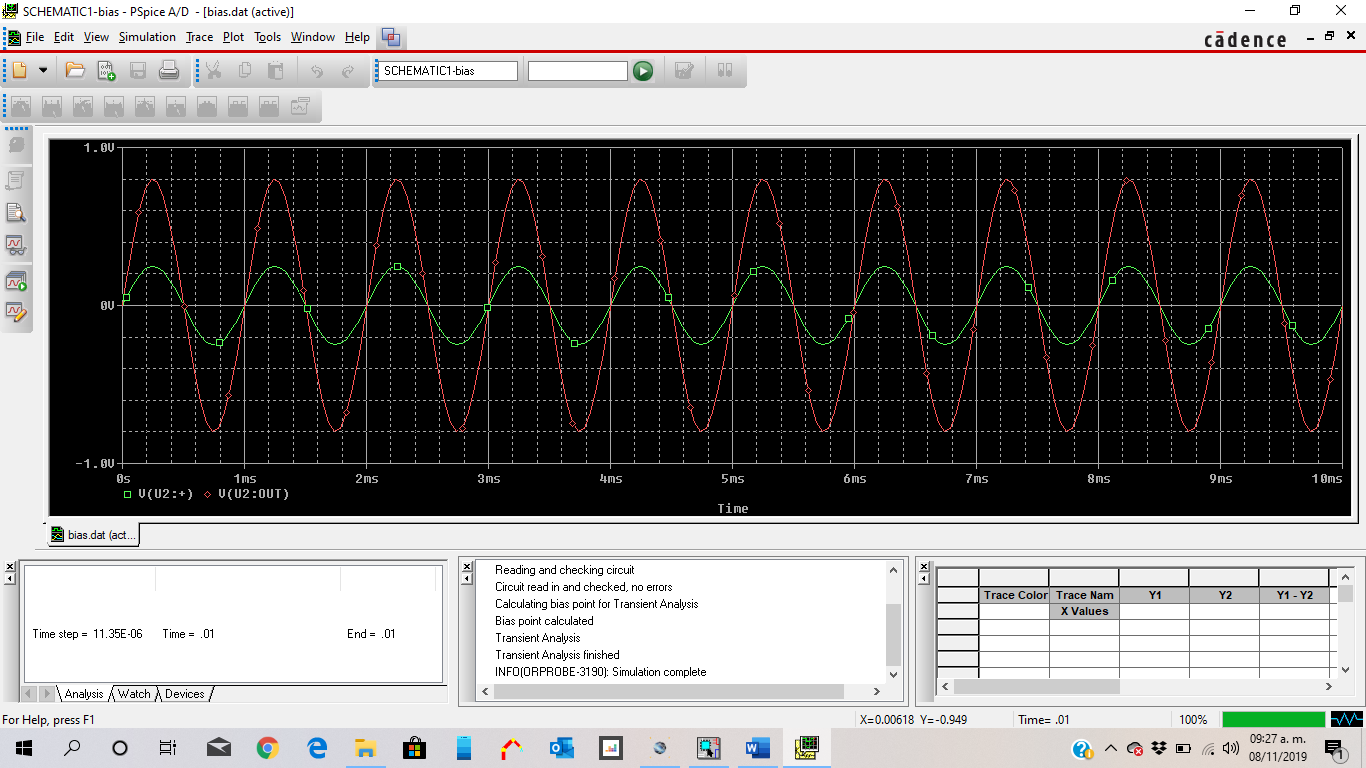
\includegraphics[scale=0.3]{4.png}
 \begin{figure}[hbtp]
 \caption{Simulacion}
 \centering
 \end{figure} 
\end{center}

En la simulacion se puede apreciar el cual es un no inversor donde tambien muestra su ganancia en donde es 2.2/1=2.2+1= \textbf{3.2} es su ganacia.



\subsection{Preguntas PCB}













\footnote{Universidad Politécnica De La Zona Metropolitana De Guadalajara} 

\newpage

\section{Tercer Circuito}
\begin{center}
 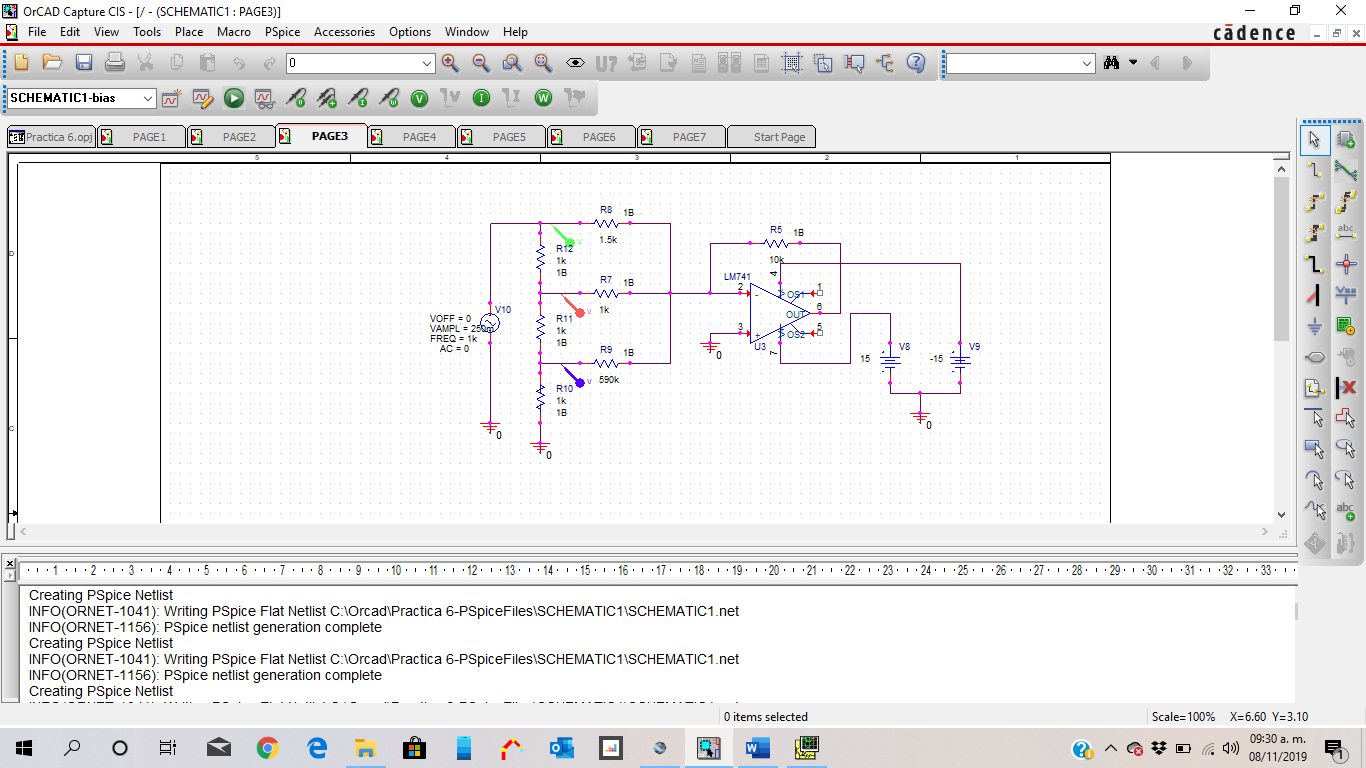
\includegraphics[scale=0.3]{5.png}
 \begin{figure}[hbtp]
 \caption{Sumador De Tres Señales Con Op Amp}
 \centering
 \end{figure}\\
  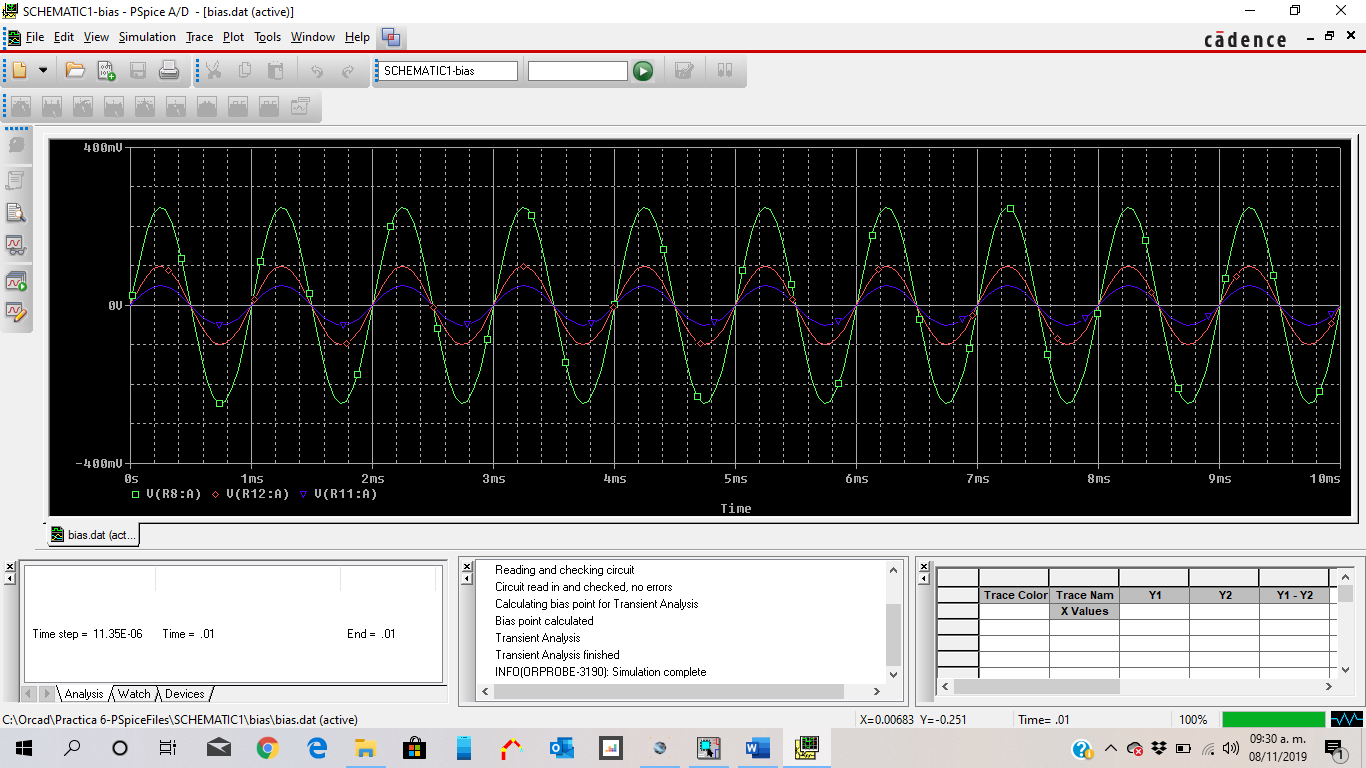
\includegraphics[scale=0.3]{6.png}
 \begin{figure}[hbtp]
 \caption{Simulacion}
 \centering
 \end{figure} 
\end{center}

En la simulacion se puede apreciar el cual es un sumador operacional donde tambien muestra sus simplitudes de cada una de las señales de cada resistencia dando su sumatorias de cada una.








\subsection{Preguntas PDF}






\footnote{Universidad Politécnica De La Zona Metropolitana De Guadalajara} 

\newpage

\section{Cuarto Circuito}
\begin{center}
 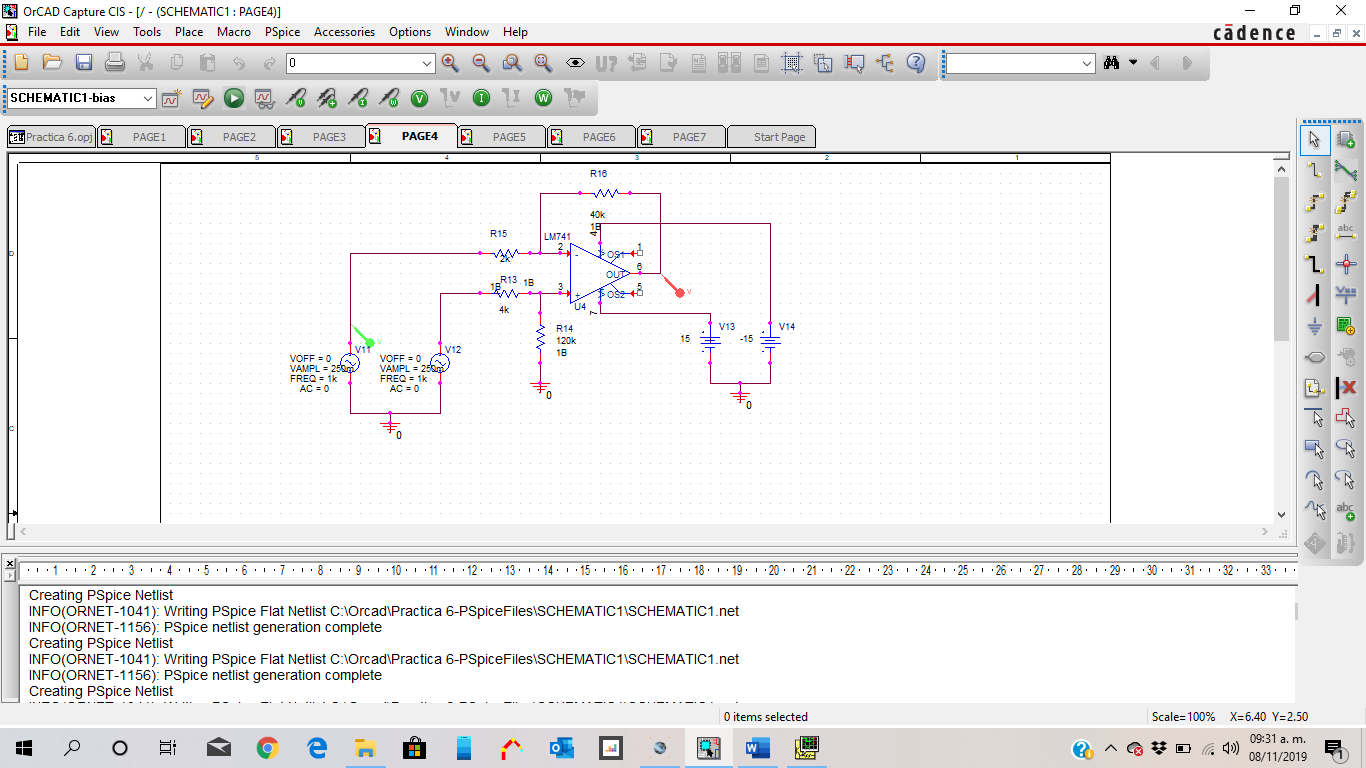
\includegraphics[scale=0.3]{7.png}
 \begin{figure}[hbtp]
 \caption{Circuito Restador Con Op Amp}
 \centering
 \end{figure}\\
  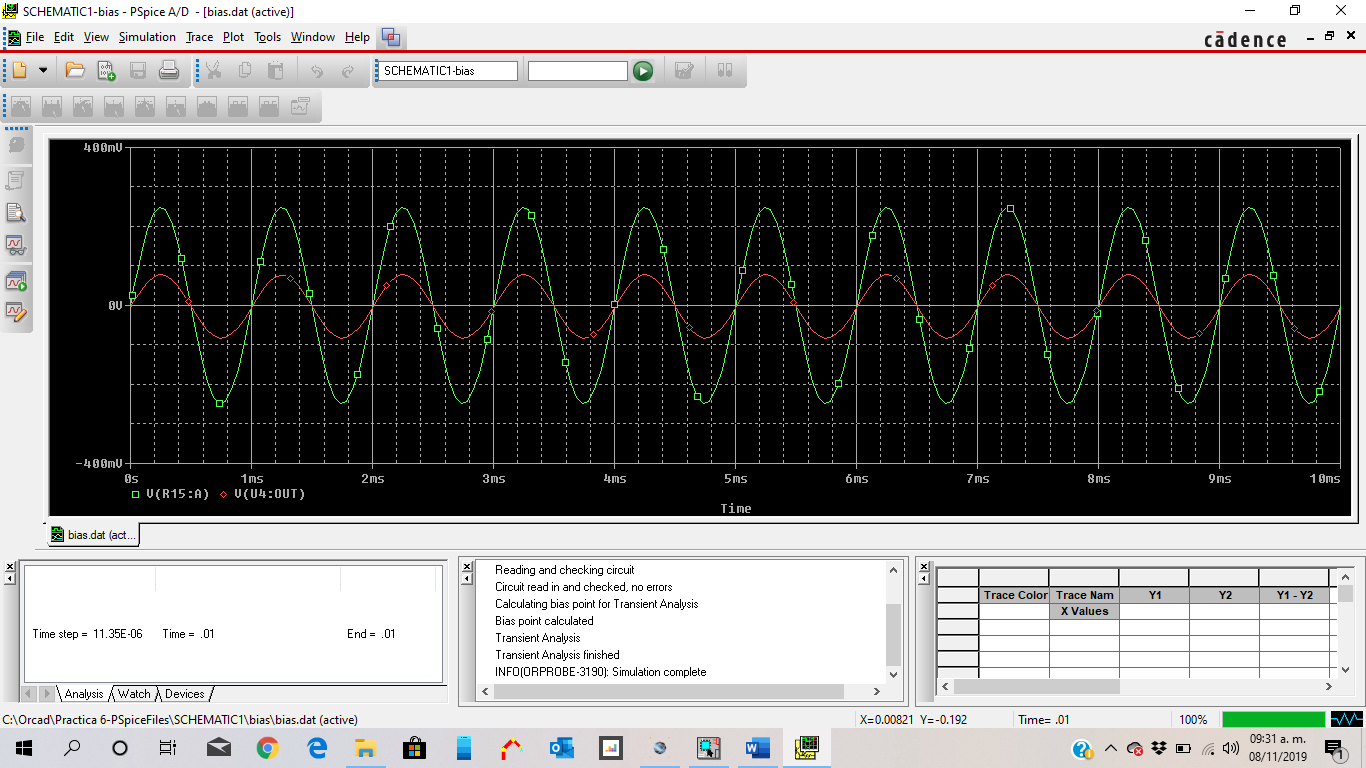
\includegraphics[scale=0.3]{8.png}
 \begin{figure}[hbtp]
 \caption{Simulacion}
 \centering
 \end{figure} 
\end{center}

En la simulacion se puede apreciar el cual es un restador operacional donde tambien muestra que seas cual sea su medicion de cualquier entrada dar la misma ya que ambas son iguales y dara tambin su onda de salida.







\subsection{Preguntas PDF}





\footnote{Universidad Politécnica De La Zona Metropolitana De Guadalajara} 

\newpage

\section{Quinto Circuito}
\begin{center}
 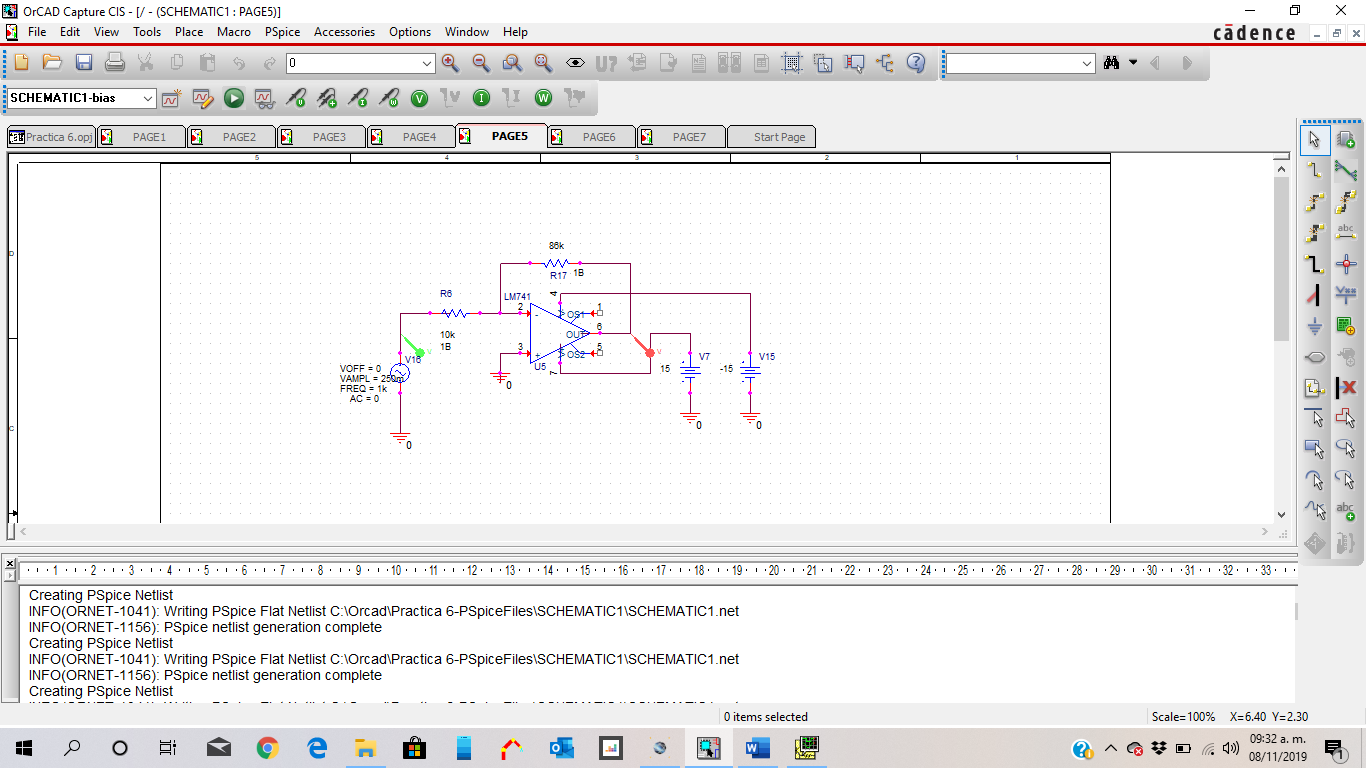
\includegraphics[scale=0.3]{9.png}
 \begin{figure}[hbtp]
 \caption{Amplificador Operacional Inversor}
 \centering
 \end{figure}\\
  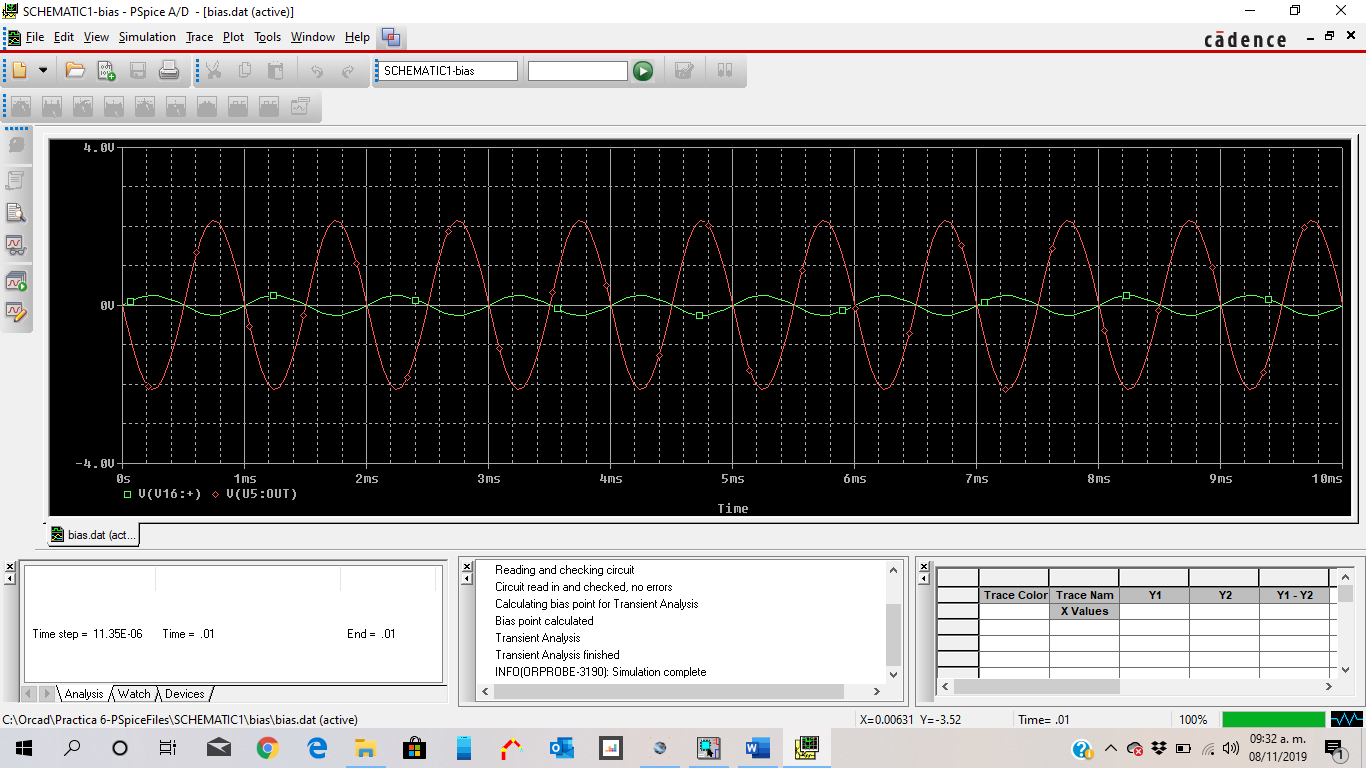
\includegraphics[scale=0.3]{10.png}
 \begin{figure}[hbtp]
 \caption{Simulacion}
 \centering
 \end{figure} 
\end{center}

En la simulacion se puede apreciar el cual es un inversor donde tambien muestra su ganancia en donde es 100/1.2= \textbf{83.33} es su ganacia.








\subsection{Preguntas PDF}





\footnote{Universidad Politécnica De La Zona Metropolitana De Guadalajara} 

\newpage

\section{Sexto Circuito}
\begin{center}
 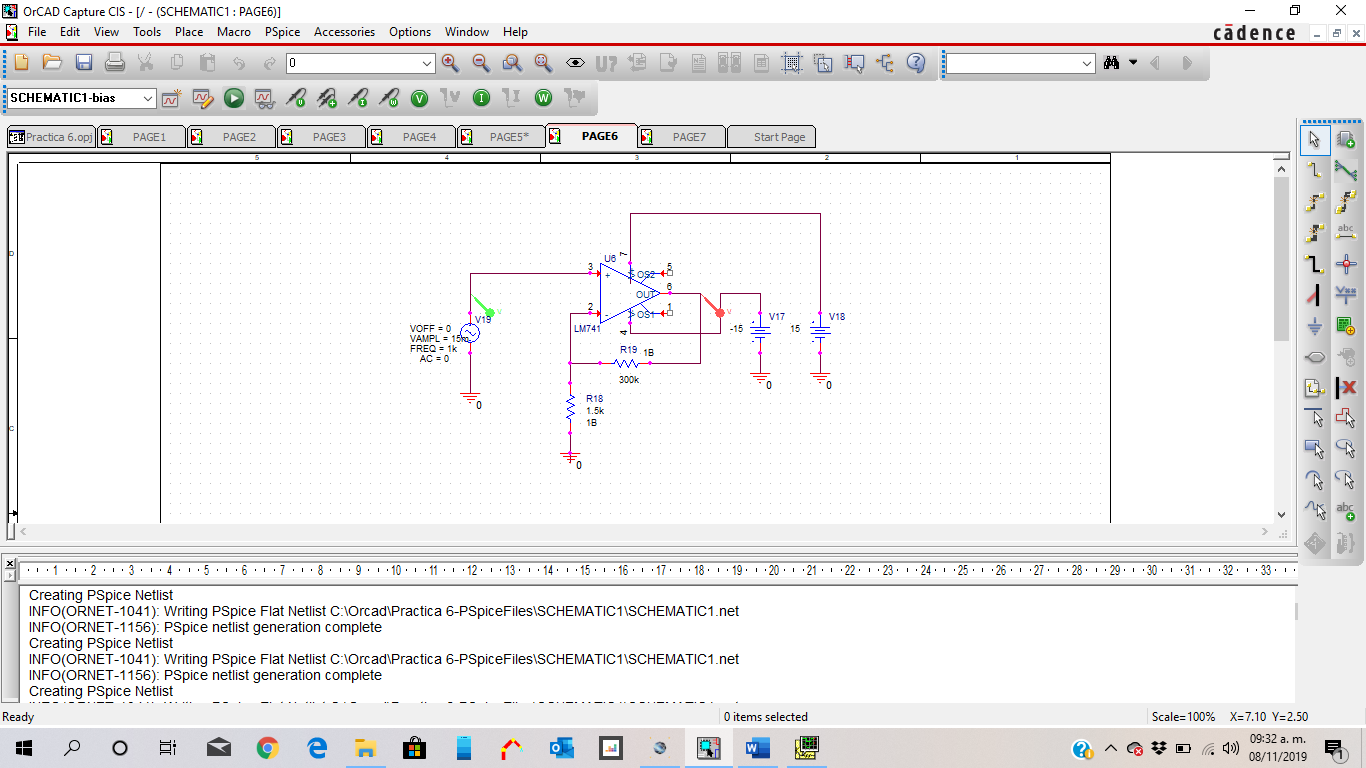
\includegraphics[scale=0.3]{11.png}
 \begin{figure}[hbtp]
 \caption{Amplificador Operacional No Inversor}
 \centering
 \end{figure}\\
  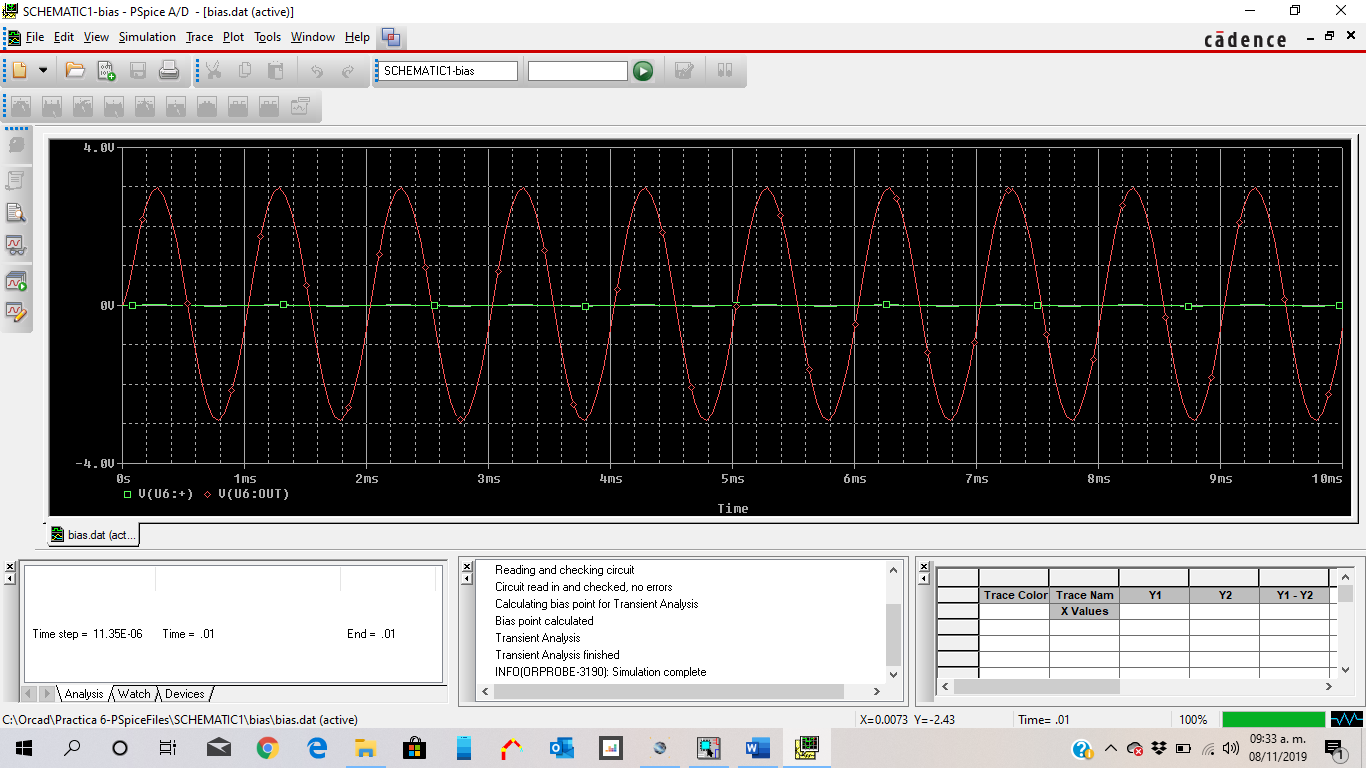
\includegraphics[scale=0.3]{12.png}
 \begin{figure}[hbtp]
 \caption{Simulacion}
 \centering
 \end{figure} 
\end{center}

En la simulacion se puede apreciar el cual es un no inversor donde tambien muestra su ganancia en donde es 300/1.5=200+1 \textbf{201} es su ganacia, en esta pudimo tener una entrada pequeña y una ganancia grande ya que solamente sencuentra 25mv.









\subsection{Preguntas PDF}


\footnote{Universidad Politécnica De La Zona Metropolitana De Guadalajara} 

\newpage

\section{Séptimo Circuito}
\begin{center}
 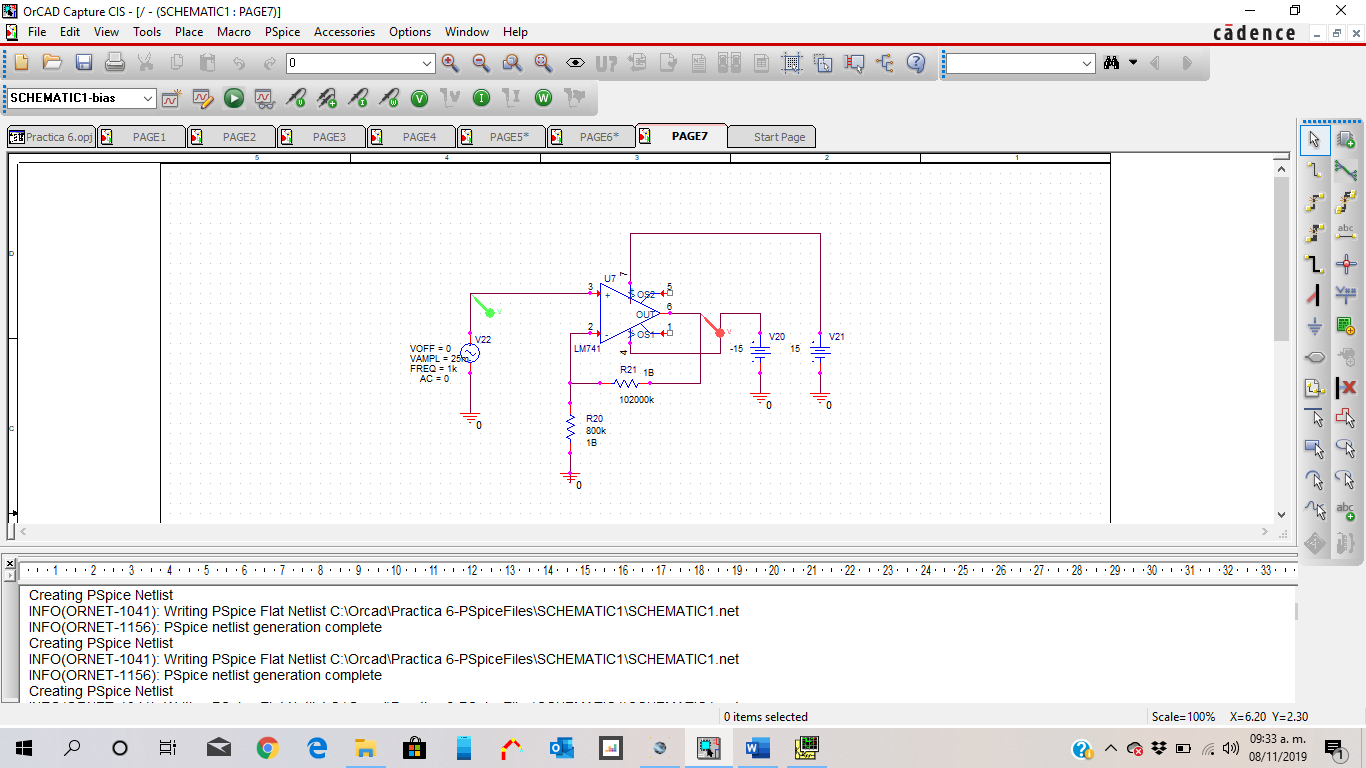
\includegraphics[scale=0.3]{13.png}
 \begin{figure}[hbtp]
 \caption{Amplificador Sumador}
 \centering
 \end{figure}\\
  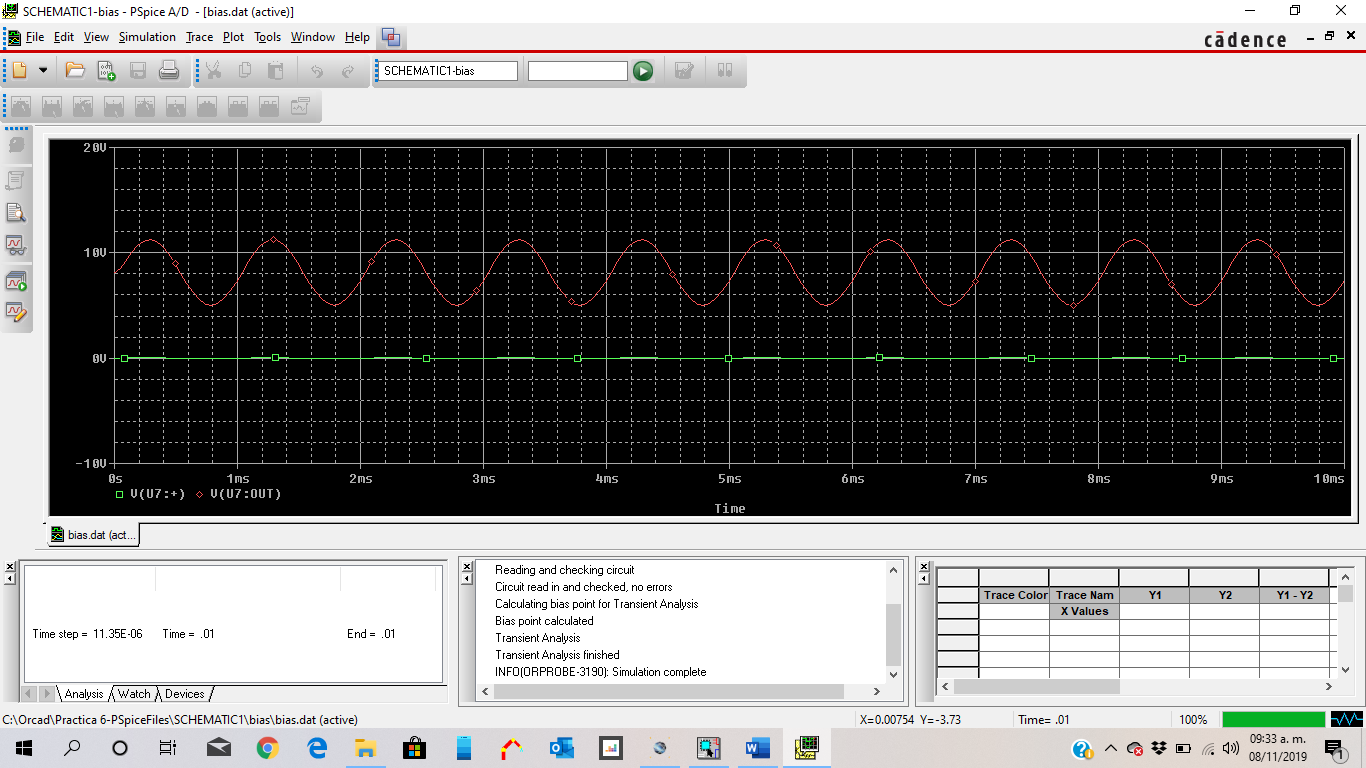
\includegraphics[scale=0.3]{14.png}
 \begin{figure}[hbtp]
 \caption{Simulacion}
 \centering
 \end{figure} 
\end{center}

En la simulacion se puede apreciar el cual es un no inversor donde tambien muestra su ganancia en donde es 102000/800=127.5+1 \textbf{128.5} es su ganancia, ya que tambien en esta pudimos tener un desface de su entrada ya que las resistencias son altas y tambien ya que son 15mv.







\subsection{Preguntas PDF}





\footnote{Universidad Politécnica De La Zona Metropolitana De Guadalajara} 

\newpage

\section{Octavo Circuito}
\begin{center}
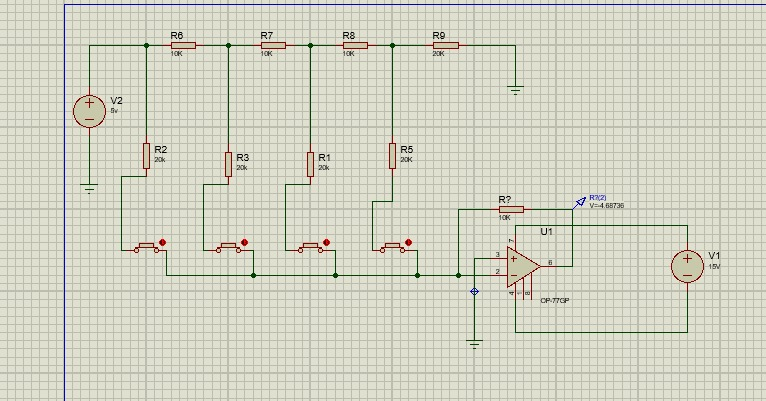
\includegraphics[scale=0.3]{15.png}
 \begin{figure}[hbtp]
 \caption{FUENTE ADC}
 \centering
 \end{figure}\\
\end{center}
Un convertidor analógico digital (ADC) es un dispositivo que convierte una cantidad física continua (generalmente voltaje) a un número digital que representan la amplitud de dicha cantidad. La conversión implica un cuantización de la entrada por lo que se produce un pequeño error al realizar la conversión.

La salida digital que produce un módulo ADC es generalmente un número binario en complemento a 2 el cual es proporcional a la entrada.

La resolución del convertidor ADC indica la cantidad de valores discretos que puede producir para representar el rango analógico de interés. Por ejemplo, una ADC de 8bits puede representar 256 niveles de una señal analógica. Para mas información ver el artículo del ADC en Wikipedia.

El conversor ADC necesita una referencia que le indique cuales son los valores máximos y mínimos de voltaje para realizar la conversión. El módulo ADC posee dos señales de referencia llamadas Voltage Reference High (V REFH) y Voltage Reference Low (V REFL) y podrá convertir muestras entre V SSAD (Tierra Analógica) y V DDAD (conectada a V REFH) que va entre 1.8 y 3.6 Volts. 
\subsection{Tabla de Bits}
0000= 0.0013V\\
0001= 0.62V\\
0010= 0.93V\\
0011= 1.25V\\
0100= 1.42V\\
0101= 1.81V\\
0110= 1.97V\\
0111= 2.18V\\
1000= 2.50V\\
1001= 3.12V\\
1010= 3.43V\\
1011= 3.75V\\
1100= 3.92V\\
1101= 4.31V\\
1110= 4.47V\\
1111= 4.68V

\footnote{Universidad Politécnica De La Zona Metropolitana De Guadalajara} 

\newpage

\section{Noveno Circuito}
\begin{center}
 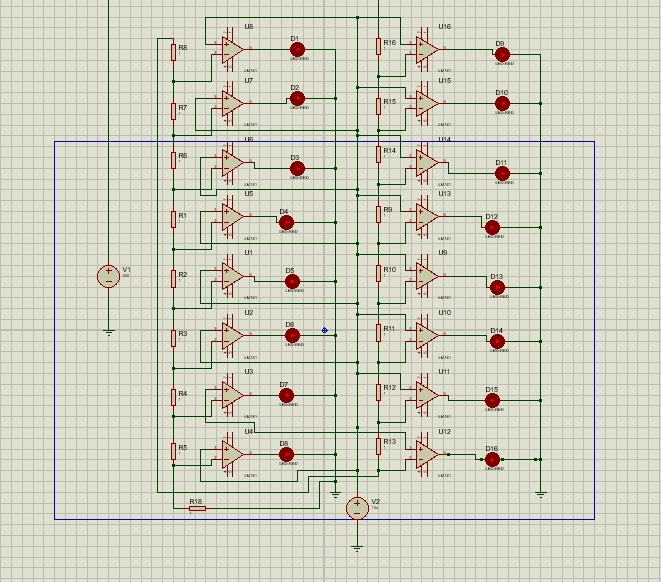
\includegraphics[scale=0.3]{16.png}
 \begin{figure}[hbtp]
 \caption{DAC}
 \centering
 \end{figure}\\
  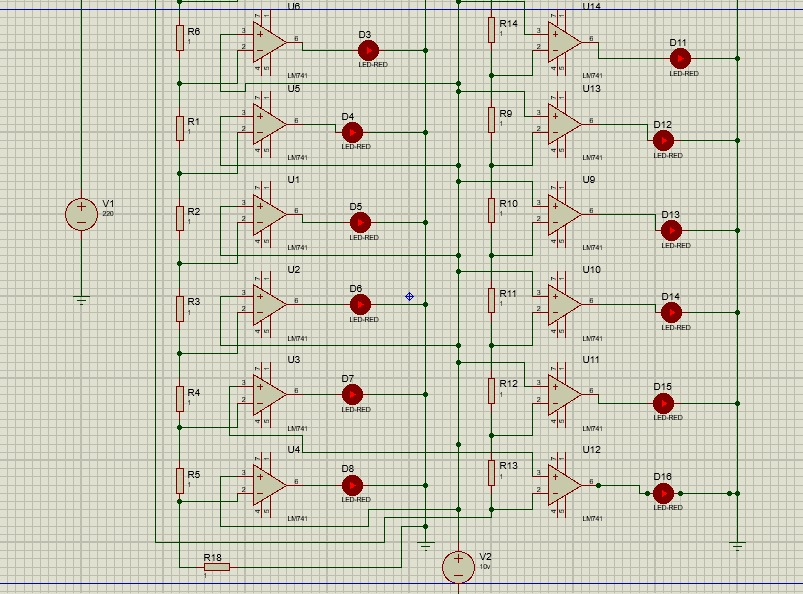
\includegraphics[scale=0.3]{17.png}
 \begin{figure}[hbtp]
 \caption{DAC}
 \centering
 \end{figure} 
\end{center}

Un conversor de señal digital a analógica o conversor digital analógico, CDA o DAC (del inglés, digital to analogue converter) es un dispositivo para convertir señales digitales con datos binarios en señales de corriente o de tensión analógica. Hay distintos componentes que pueden intervenir en este proceso, como interruptores simples, red de resistores, fuentes actuales o condensadores. Un convertidor de analógico a digital (ADC) realiza la operación inversa.

Las señales en la naturaleza tienen las características de ser continuas en su magnitud y en el diagrama temporal. La digitalización es necesaria para el procesamiento, almacenamiento y filtrado de señales analógicas con los beneficios que las señales digitales conllevan, como mayor inmunidad al ruido, circuitos electrónicos más simples para el procesamiento y almacenamiento. Representación unívoca de los elementos, cuya cantidad de símbolos es proporcional a 2n, siendo n la cantidad de bits.

\footnote{Universidad Politécnica De La Zona Metropolitana De Guadalajara} 

\newpage

\subsection{Tabla de Bits}
Led's    Volts\\
 0 =      210v\\
 1 =      200v\\
 2 =      190v\\
 3 =      180v\\
 4 =      160v\\
 5 =      150v\\
 6 =      140v\\
 7 =      120v\\
 8 =      110v\\
 9 =      100v\\
 10 =     80v\\
 11 =     70v\\
 12 =     60v\\
 13 =     50v\\
 14 =     30v\\
 15 =     20v

\section{Conclusiones}

En el desarrollo de esta practica aprendí como desarrollar circuitos amplificadores tanto con señales -inversas como no-inversas y que algunas estén amplificadas como restadas. Estos circuitos nos permiten tener ganancias dependiendo el que hallas armado pero haciendo la función por el cual es nombrado, por ejemplo el inversor podremos observar que la señal esta invertida respecto la entrada con la salida y que también tenemos un ganancia restando el valor de entrada por el de salida con las resistencias correspondientes usando formula como la de retroalimentación o la misma de ganancia. También al final tenemos dos convertidores aplicando comandos de 1 y 0 los cuales nos dan diferentes valores o también nos permiten encender leds con entradas de voltaje diferente convirtiendo valores de entrada ya se 0 y 1 o el voltaje con el adc aprovechar diferentes voltajes en las salidas.




\bibliographystyle{https://es.wikipedia.org/wiki/Amplificador_operacional\
https://www.electronicafacil.net/tutoriales/AMPLIFICADOR-INVERSOR.html\
http://www.electronicasi.com/ensenanzas/electronica-avanzada/electronica-universitaria/electronica-analogica/amplificador-no-inversor/\
http://hyperphysics.phy-astr.gsu.edu/hbasees/Electronic/opampvar6.html\
https://unicrom.com/amplificador-sumador-con-amplificadores-operacionales/}


\footnote{Universidad Politécnica De La Zona Metropolitana De Guadalajara} 



\end{document}